\documentclass[a4paper,11pt]{article}
\author{ 杨旭鹏  \  PB17000234}
\date{2019年秋季}
\title{计算物理A 第十八题}

\usepackage{ctex}
\usepackage{amsmath}
\usepackage{amsfonts}
\usepackage{graphicx}
\usepackage{lastpage}
\usepackage{hyperref}
\usepackage{appendix}
\usepackage{geometry}
\geometry{left=2.5cm,right=2.5cm,top=2.5cm,bottom=2.5cm}
\makeatletter\def\@captype{table}\makeatother
\usepackage{enumerate}
\usepackage{listings}
\RequirePackage{xcolor}
 
\definecolor{dkgreen}{rgb}{0,0.6,0}
\definecolor{gray}{rgb}{0.5,0.5,0.5}
\definecolor{mauve}{rgb}{0.58,0,0.82}

\lstset{
  frame=tb,
  aboveskip=3mm,
  belowskip=3mm,
  showstringspaces=false,
  columns=flexible,
  framerule=1pt,
  rulecolor=\color{gray!35},
  backgroundcolor=\color{gray!5},
  basicstyle={\small\ttfamily},
  numbers=left,
  numberstyle=\tiny\color{gray},
  keywordstyle=\color{blue},
  commentstyle=\color{dkgreen},
  stringstyle=\color{mauve},
  breaklines=true,
  breakatwhitespace=true,
  tabsize=3,            
  }



\begin{document}
\maketitle

\section{题目描述}
设计一个MPI程序,满足:
\begin{enumerate}
	\item 各进程随机生成一个 10$\times$10 二维单精度浮点数组,且各进程中的数组对应元素值的不全一样 
	\item 调用集合通信 MPI\_Reduce 函数实现对数组中对应元素求最大值的归约操作
	\item 利用点对点通讯实现上述归约操作并与其进行验证
\end{enumerate}

编译、测试运行可使用 https://training.ustc.edu.cn/ 中的《MPI编译环 境的使用》

\section{程序思路}
首先初始化并行环境 MPI\_Init 。在主进程中产生供不同进程使用的不同随机种子,存在一个数组中,利用集合通信(MPI\_Bcast)将此数组共享给其他进程。然后利用循环对所有位置的矩阵元求最大值,利用两种方法求某位置矩阵元的最大值:
\begin{enumerate}
	\item 利用集合通信:将每一进程的某矩阵元传入 MPI\_Reduce 函数,并发送到最后一个进程中,设定 MPI\_Op 操作为为 MPI\_MAX,然后在最后一个进程中打印传入的寻找到的最大值矩阵即为所求。
	\item 利用点对点通信:将每一非最后一个进程中的某矩阵元数值传入最后一个进程中,在最后一个进程接收到一数组中,然后比较数组中的元素,将最大值存入某数组,打印,即为所求。
\end{enumerate}

\section{程序说明}
该程序中矩阵元均为$(0,1)$的随机单精度浮点数,且初始种子与时间有关,故此程序每次运行结果均不同。按照老师给的示例,需要将所有的矩阵打印出来,为了保证进程间打印不互相干扰,故程序设有打印的标志flag,标志值不为0时才执行打印操作。初始只有主进程flag不为0,其余进程打印之前接受上一进程传来的flag置1信号。打印完成之后利用点对点通信将下一个进程的flag置1,以完成顺序打印随机矩阵。

编译命令为:mpicc −o mpi mpi.c,运行命令按照李老师给的示例为:mpirun -n 4 ./mpi ,默认开启4个进程。

\section{程序结果}
将本程序源代码文件“mpi.c”上传到中国科大计算实训平台上,然后编译运行。得到如下结果:


\begin{figure}[!htbp]
\centering
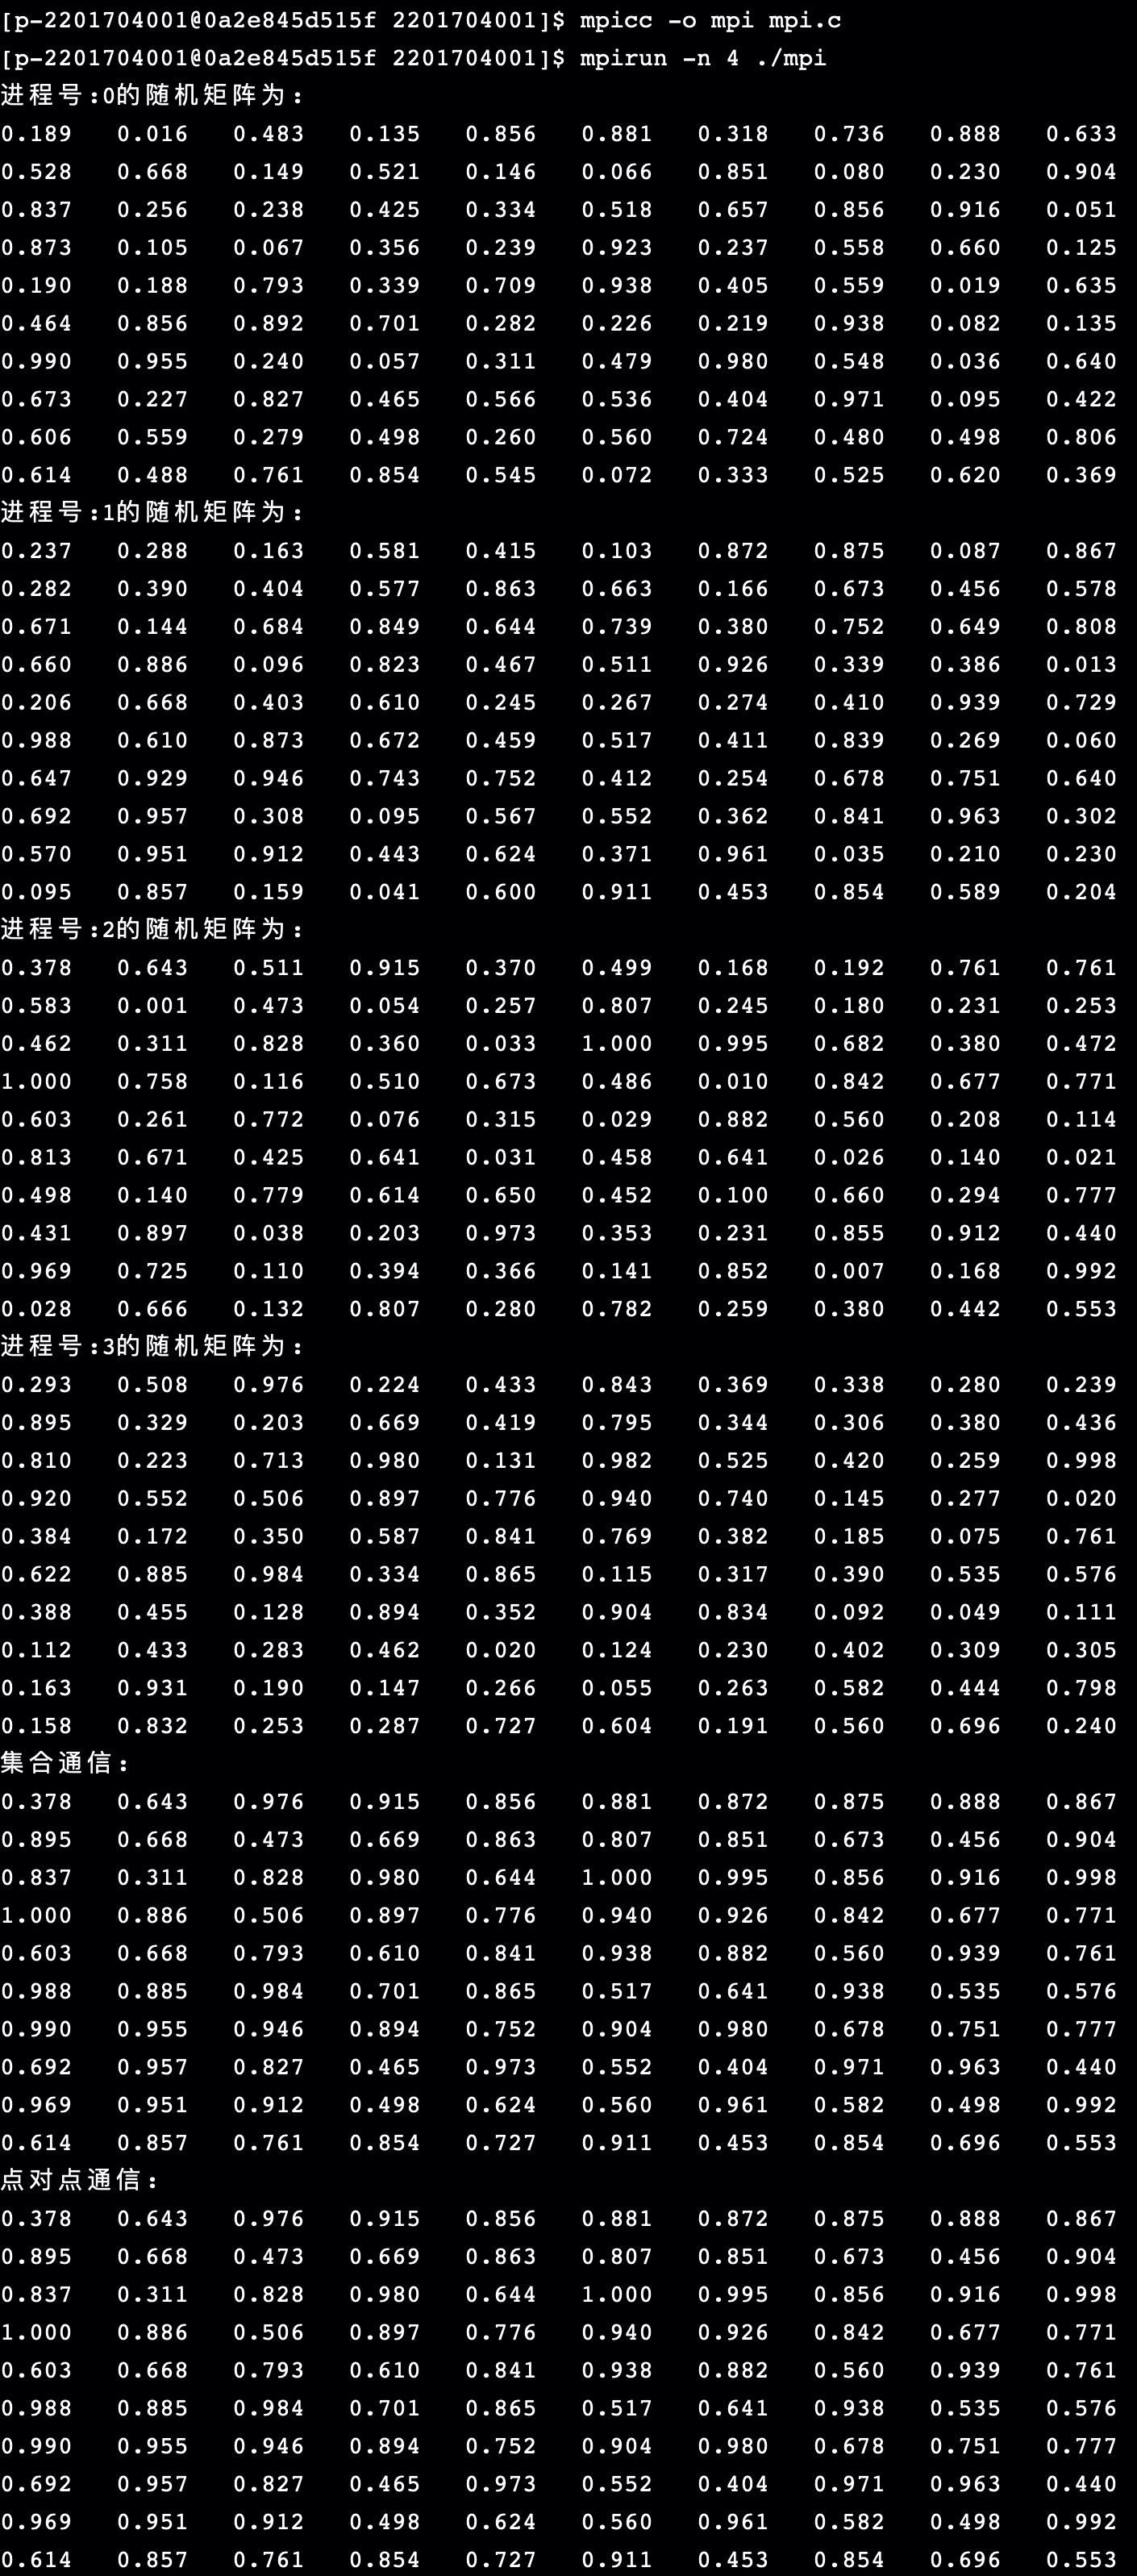
\includegraphics[width = 9cm]{result.jpg}
\caption{程序运行过程示意}	
\end{figure}

其中,最后输出的2个矩阵分别为两种方式求得的最大值矩阵。可以看出两个方法均能求出最大值矩阵。程序成功。

\section{心得体会}
虽然本次作业思路上相比之前的作业简单不少,但是毕竟是对新的语法进行编程,花费的时间也不算太少。编程中发现MPI\_Reduce函数应在每个进程中都运行,一开始只在一个进程中运行发现结果上有问题。还有就是程序间打印顺序的问题也调试了很久。总之确实是熟悉了一下MPI的基本语法。

\section{C语言程序源代码}
\begin{lstlisting}[language = C]
#include <stdio.h>
#include <string.h>
#include <stdlib.h>
#include <time.h>
#include "mpi.h"
#define GETMATELEM(base,i,j,imax) ((*(base + (i) * (imax) + (j)))) //取二维数组元素


int matrixform(float *matrix,int m,int n){  //打印矩阵的函数
    int i,j;
    for(i=0;i<m;i++){
        for(j=0;j<n;j++){
            printf("%.3f\t", GETMATELEM(matrix,i,j,n) );
        }
        printf("\n");
    }
    return 0;
}



int main(int argc, char* argv[]){
    
    int m;  //求最大值的矩阵元行位置
    int n;  //求最大值的矩阵元列位置
    float *max1 = malloc(sizeof(float)*100); //利用集合通信求得的最大值矩阵
    float *max2 = malloc(sizeof(float)*100); //利用点对点通信求得的最大值矩阵
    int flag = 0; //打印矩阵的标志
    int one = 1;  //值为 (int) 1 的变量
    
    int numprocs, myid, source;
    MPI_Status status;
    MPI_Init(&argc,&argv);
    MPI_Comm_rank(MPI_COMM_WORLD, &myid);
    MPI_Comm_size(MPI_COMM_WORLD, &numprocs);
    
    float *max2temp = malloc(sizeof(float)*numprocs);  //点对点通信时比较大小所用的临时数组
    unsigned int seed[numprocs];  //随机种子数组
    
    if(myid == 0){
        
        time_t t;
        srand((unsigned) time(&t));
        int i;
        for(i=0;i < numprocs;i++){  //种子初始化
            seed[i] = rand();
        }
        srand(seed[myid]);
        flag = 1;
        
    }
    
    MPI_Bcast(seed, numprocs, MPI_UNSIGNED, 0, MPI_COMM_WORLD);  //广播主进程求得的随机种子数组
   
    srand(seed[myid]);          //对不同进程赋不同的随机种子
    float *matrix = malloc(sizeof(float)*100);       //为每一个进程定义随机矩阵
    int j,k;
    for(j=0;j<10;j++){      //对随机矩阵赋值
        for(k=0;k<10;k++){
            GETMATELEM(matrix,j,k,10) = rand()/(float)RAND_MAX;  //矩阵元为(0,1)随机f单精度浮点数
        }
    }
    
    
    if(myid != 0){
        MPI_Recv(&flag, 1, MPI_INT, myid -1 , 1, MPI_COMM_WORLD, &status);//接受上一个进程传入的打印矩阵flag参数
    }
    
    
    if(flag != 0){   //若打印flag不为0,则执行打印矩阵命令
        printf("进程号:%d的随机矩阵为:\n",myid);
        matrixform(matrix,10,10);
        if(myid < numprocs -1){
            MPI_Send(&one, 1, MPI_INT, myid + 1, 1, MPI_COMM_WORLD);  //向下一个进程传入的打印矩阵flag参数
        }
    }
   
        
    
    for(m=0;m<10;m++){   //对矩阵行元素循环
           for(n=0;n<10;n++){  //对矩阵列元素循环
               MPI_Reduce(&GETMATELEM(matrix,m,n,10), &GETMATELEM(max1,m,n,10), 1, MPI_FLOAT, MPI_MAX, numprocs-1, MPI_COMM_WORLD); //集合通信求最大值矩阵
               
               if(myid != numprocs -1){
                   MPI_Send(&GETMATELEM(matrix,m,n,10), 1, MPI_FLOAT, numprocs -1, myid+10, MPI_COMM_WORLD); // 点对点通信
               }
               
               if(myid == numprocs-1){  //最后一个进程中利用点对点通信求最大值
                   int i;
                   GETMATELEM(max2,m,n,10) = GETMATELEM(matrix,m,n,10);
                   for(i = 0;i<numprocs-1;i++){    //点对点接受然后求最大值
                        MPI_Recv(&max2temp[i], 1, MPI_FLOAT, i, i+10, MPI_COMM_WORLD, &status);
                        if(max2temp[i] > GETMATELEM(max2,m,n,10) ){
                            GETMATELEM(max2,m,n,10) = max2temp[i];
                        }
                    }
                   
               }
           }
       }
     
    
    if(myid == numprocs-1){  //最后一个进程打印最大值矩阵
        printf("集合通信:\n");
        matrixform(max1,10,10);
        printf("点对点通信:\n");
        matrixform(max2,10,10);
    }
        
    MPI_Finalize();
}

	
\end{lstlisting}














\end{document}